%!TEX TS-program = xelatex
%!TEX encoding = UTF-8 Unicode
\documentclass[12pt,a4paper]{article}

\usepackage{graphicx}
\usepackage{float}
\usepackage{caption}
\usepackage{subcaption}
\usepackage{geometry}
\usepackage{fancyhdr}
\setlength{\headheight}{14pt}
\usepackage{xcolor}
\usepackage[hidelinks]{hyperref}
\usepackage{listings}
\usepackage{xepersian}

\geometry{margin=2.5cm}

\settextfont{Vazirmatn UI}
\setlatintextfont{FreeSerif}
\setdigitfont{Vazirmatn UI}

\pagestyle{fancy}
\fancyhf{}
\fancyhead[L]{\small پروژه سوم - پیاده‌سازی الگوریتم اجماع Raft}
\fancyfoot[C]{\thepage}
\renewcommand{\headrulewidth}{0.4pt}

\lstset{
    basicstyle=\ttfamily\small,
    backgroundcolor=\color{gray!10},
    frame=single,
    breaklines=true,
    numbers=left,
    numberstyle=\tiny,
    showstringspaces=false
}

\begin{document}

\begin{titlepage}
    \centering
    \vspace*{2cm}
    
    {\huge\bfseries گزارش پروژه سیستم‌های توزیع‌شده}
    
    \vspace{1cm}
    {\Large پروژه سوم: پیاده‌سازی الگوریتم اجماع \lr{Raft}}
    
    \vspace{2cm}
    
    \begin{tabular}{lr}
 
       \textbf{اعضای تیم:} & \\
        & محمد سعید صدیقی - ۸۱۰۱۰۰۱۷۹ \\
        & محمد حسین مطاعی - ۸۱۰۱۹۹۴۹۳ \\
        & محمد مهدی خصالی - ۸۱۰۱۰۰۱۳۴ \\
    \end{tabular}
    
    \vfill
    
    {\large دانشگاه تهران - دانشکده مهندسی کامپیوتر}
    \\
    {\large بهار ۱۴۰۴}
\end{titlepage}

\tableofcontents
\newpage

\section{مقدمه}

این گزارش به تفصیل به پیاده‌سازی الگوریتم اجماع \lr{Raft} در چارچوب یک پروژه 
درس سیستم‌های توزیع‌شده می‌پردازد. الگوریتم \lr{Raft} یک پروتکل اجماع طراحی شده برای مدیریت لاگ‌های تکرار شده \lr{(Replicated Log)} در سیستم‌های توزیع‌شده است.
هدف اصلی این الگوریتم، فراهم آوردن تحمل‌پذیری در برابر خرابی \lr{(Fault Tolerance)} و حفظ سازگاری \lr{(Consistency)} داده‌ها در میان چندین سرور است، حتی زمانی که برخی از سرورها از کار می‌افتند یا شبکه ناپایدار می‌شود.
\lr{Raft} به عنوان جایگزینی قابل فهم‌تر برای الگوریتم‌های خانواده \lr{Paxos} طراحی شده است.
این قابلیت فهم بالا از طریق تفکیک منطق به اجزای مستقل‌تر مانند انتخاب رهبر، تکرار لاگ و تضمین‌های ایمنی حاصل می‌شود.
با وجود سادگی بیشتر در درک، \lr{Raft} از نظر کارایی با \lr{Paxos} قابل مقایسه است و ایمنی آن به صورت رسمی اثبات شده است.
این الگوریتم با سازماندهی درخواست‌های مشتری به صورت یک توالی مشخص به نام «لاگ» \lr{(Log)} و اطمینان از اینکه تمامی سرورها نسخه‌ای یکسان از این لاگ را مشاهده می‌کنند، سازگاری را تضمین می‌کند.
پروژه حاضر شامل پیاده‌سازی الگوریتم \lr{Raft} به صورت یک شیء \lr{Go} با توابع مرتبط است، به گونه‌ای که نمونه‌های مختلف \lr{Raft} بتوانند از طریق \lr{RPC} با یکدیگر ارتباط برقرار کرده و لاگ‌ها را هماهنگ نگه دارند.
این پیاده‌سازی بر سه بخش کلیدی الگوریتم \lr{Raft} متمرکز بوده است: انتخاب رهبر \lr{(Leader Election)} که در بخش \lr{3A} مورد بررسی قرار گرفت، ثبت لاگ \lr{(Log Replication)} که مربوط به بخش \lr{3B} است، و پایداری \lr{(Persistence)} که در بخش \lr{3C} پیاده‌سازی شد.
لازم به ذکر است که بخش فشرده‌سازی لاگ \lr{(Log Compaction)} که به عنوان بخش \lr{3D} در دستورالعمل پروژه ذکر شده بود، در این پیاده‌سازی انجام نشده و بنابراین در این گزارش به آن اشاره‌ای نخواهد شد.
انتخاب \lr{Raft} برای این پروژه دانشگاهی در درس سیستم‌های توزیع‌شده، یک تصمیم آگاهانه آموزشی است.
تأکید \lr{Raft} بر قابل فهم بودن و تجزیه واضح مسائل اجماع (مانند انتخاب رهبر، تکرار لاگ و ایمنی) فرآیند یادگیری را برای دانشجویان تسهیل می‌کند و به آن‌ها کمک می‌کند تا مفاهیم پیچیده اجماع توزیع‌شده را به خوبی درک کنند. ما برای این پروژه از یک روز گریس استفاده کردیم.

\section{معماری سیستم Raft}

الگوریتم \lr{Raft} بر اساس مجموعه‌ای از سرورها بنا شده است که با همکاری یکدیگر، یک سرویس تکرار شده \lr{(Replicated Service)} را ارائه می‌دهند. این سرویس با نگهداری نسخه‌های کامل از وضعیت داده‌ها در چندین سرور، تحمل‌پذیری در برابر خرابی را فراهم می‌آورد. در هسته معماری \lr{Raft}، سه نقش اصلی برای سرورها تعریف شده است که هر سرور در هر لحظه در یکی از این حالت‌ها قرار دارد: رهبر \lr{(Leader)}، پیرو \lr{(Follower)} و کاندیدا \lr{(Candidate)}.

\subsection{اجزای کلیدی Raft}

\begin{itemize}
    \item \textbf{سرورها و حالت‌ها:}
    \begin{itemize}
        \item \textbf{پیرو \lr{(Follower)}:} این حالت، وضعیت پیش‌فرض و منفعل یک سرور است. پیروها تنها به درخواست‌های رهبر یا کاندیداها پاسخ می‌دهند. اگر یک پیرو برای مدت زمان مشخصی که به آن «زمان‌بندی انتخابات» \lr{(election timeout)} گفته می‌شود، هیچ پیامی از رهبر دریافت نکند، فرض می‌کند که رهبر از کار افتاده و وضعیت خود را به کاندیدا تغییر می‌دهد.
        \item \textbf{کاندیدا \lr{(Candidate)}:} سروری که از حالت پیرو به این حالت تغییر وضعیت داده است، به این معنی که قصد دارد رهبر جدید کلاستر شود. با آغاز یک دوره \lr{(Term)} جدید، کاندیدا ابتدا به خودش رأی می‌دهد و سپس درخواست‌های رأی \lr{(RequestVote RPCs)} را به سایر سرورها ارسال می‌کند تا حمایت آن‌ها را جلب کند.
        \item \textbf{رهبر \lr{(Leader)}:} تنها یک رهبر در هر کلاستر \lr{Raft} در یک زمان مشخص وجود دارد. رهبر مسئول اصلی پذیرش درخواست‌های مشتری، تکرار ورودی‌های لاگ به تمامی پیروها، و ارسال منظم پیام‌های ضربان قلب \lr{(Heartbeat)} برای حفظ رهبری خود و جلوگیری از آغاز انتخابات جدید است.
    \end{itemize}
    \item \textbf{گذار حالت \lr{(State Transition)}:}
    \begin{itemize}
        \item \textbf{پیرو به کاندیدا:} زمانی اتفاق می‌افتد که زمان‌بندی انتخابات منقضی شود و هیچ پیام \lr{Heartbeat} از رهبر دریافت نشود.
        \item \textbf{کاندیدا به رهبر:} زمانی رخ می‌دهد که کاندیدا اکثریت آرا را از سرورهای دیگر کلاستر دریافت کند.
        \item \textbf{کاندیدا به پیرو:} اگر کاندیدا یک پیام \lr{AppendEntries RPC} یا \lr{RequestVote RPC} با یک \lr{Term} بالاتر از \lr{Term} فعلی خود دریافت کند، بلافاصله به حالت پیرو بازمی‌گردد.
        \item \textbf{رهبر به پیرو:} اگر رهبر یک \lr{RPC} با \lr{Term} بالاتر از \lr{Term} فعلی خود دریافت کند، به حالت پیرو تغییر وضعیت می‌دهد.
    \end{itemize}
    \item \textbf{لاگ \lr{(Log)}:} لاگ یک توالی مشخص از دستورات \lr{(Commands)} است که تمامی سرورها باید نسخه‌ای یکسان از آن را داشته باشند. هر سرور دستورات را به ترتیب در لاگ خود اعمال می‌کند تا وضعیت یکسانی را در سراسر کلاستر حفظ کند.
    \item \textbf{\lr{RPC}ها \lr{(Remote Procedure Calls)}:} ارتباط بین نمونه‌های \lr{Raft} به صورت انحصاری از طریق \lr{RPC} انجام می‌شود و استفاده از متغیرهای اشتراکی بین نمونه‌ها مجاز نیست. دو نوع \lr{RPC} اصلی در \lr{Raft} وجود دارد:
    \begin{itemize}
        \item \lr{RequestVote}: توسط کاندیداها برای جمع‌آوری آرا در طول انتخابات ارسال می‌شود.
        \item \lr{AppendEntries}: توسط رهبر برای تکرار ورودی‌های لاگ و همچنین به عنوان پیام \lr{Heartbeat} برای اعلام حضور خود به پیروها استفاده می‌شود.
    \end{itemize}
\end{itemize}

\subsection{مفاهیم Term و Log Entry}

\begin{itemize}
    \item \textbf{\lr{Term} (دوره):} \lr{Term} یک دوره زمانی منطقی و دلخواه در سرور است که با هر انتخابات رهبر جدید آغاز می‌شود. شماره \lr{Term} به صورت یکنواخت افزایش می‌یابد و در تمامی ارتباطات \lr{RPC} بین سرورها مبادله می‌شود. این مفهوم به \lr{Raft} کمک می‌کند تا ناهماهنگی‌های زمانی را مدیریت کرده و یک ترتیب جهانی برای رویدادها فراهم کند. مکانیزم \lr{Term} در \lr{Raft} به عنوان یک ساعت منطقی حیاتی و یک مکانیزم ایمنی اصلی عمل می‌کند. افزایش یکنواخت آن و قانون بازگشت سرورها به حالت پیرو در صورت مشاهده \lr{Term} بالاتر، به صورت بنیادی حل تعارضات را ساده کرده و سازگاری در سراسر کلاستر را تضمین می‌کند. این ویژگی، سنگ بنای مقاومت \lr{Raft} در برابر تقسیم‌بندی شبکه و خرابی سرورها را تشکیل می‌دهد.
    \item \textbf{\lr{Log Entry} (ورودی لاگ):} هر \lr{Log Entry} شامل یک دستور \lr{(Command)} است که باید توسط ماشین حالت اجرا شود، و همچنین \lr{Term} مربوط به زمانی که این ورودی توسط رهبر دریافت شده است. ورودی‌ها به صورت اعدادی با شماره ایندکس \lr{(Index)} ذخیره می‌شوند و هر ورودی معتبر باید وارد لاگ شده و سپس به سیستم بزرگتر تحویل داده شود.
\end{itemize}

\section{پیاده‌سازی انتخاب رهبر (بخش 3A)}

پیاده‌سازی بخش \lr{3A} بر مکانیزم انتخاب رهبر در الگوریتم \lr{Raft} و همچنین پیاده‌سازی پیام‌های \lr{Heartbeat} تمرکز دارد. این بخش برای تضمین وجود یک هماهنگ‌کننده فعال و پاسخگو در کلاستر حیاتی است.

\subsection{توضیح مکانیزم انتخاب رهبر و نقش Heartbeatها}

فرآیند انتخاب رهبر در \lr{Raft} به شرح زیر است: هنگامی که یک پیرو برای مدت زمان مشخصی که به آن «زمان‌بندی انتخابات» \lr{(election timeout)} گفته می‌شود، هیچ پیامی از رهبر دریافت نمی‌کند، فرض می‌کند که رهبر فعلی از کار افتاده یا ارتباطش قطع شده است. در این حالت، پیرو وضعیت خود را به کاندیدا تغییر می‌دهد. کاندیدا \lr{Term} خود را افزایش می‌دهد، به خودش رأی می‌دهد و سپس \lr{RPC}های \lr{RequestVote} را به سایر سرورها در کلاستر ارسال می‌کند تا رأی آن‌ها را جلب کند. اگر کاندیدا بتواند اکثریت آرا را از سرورهای دیگر دریافت کند، به رهبر جدید کلاستر تبدیل می‌شود.

پس از انتخاب شدن، رهبر شروع به ارسال منظم پیام‌های \lr{Heartbeat} به تمامی پیروهای خود می‌کند. این \lr{Heartbeat}ها در واقع پیام‌های \lr{AppendEntries} هستند که محتوای لاگ خالی دارند. هدف اصلی این پیام‌ها، حفظ رهبری رهبر فعلی و جلوگیری از آغاز انتخابات‌های جدید توسط پیروها است. دریافت منظم \lr{Heartbeat}ها توسط پیروها، تایمر \lr{election timeout} آن‌ها را بازنشانی می‌کند و از تغییر وضعیت آن‌ها به کاندیدا جلوگیری می‌کند.

\subsection{جزئیات پیاده‌سازی RPCهای RequestVote و AppendEntries}

پیاده‌سازی این بخش شامل تکمیل ساختارهای \lr{RequestVoteArgs} و \lr{RequestVoteReply} برای تبادل اطلاعات در طول فرآیند رأی‌گیری است. \lr{RequestVoteArgs} شامل اطلاعاتی مانند \lr{Term} کاندیدا، شناسه کاندیدا، ایندکس آخرین ورودی لاگ و \lr{Term} آخرین ورودی لاگ است. \lr{RequestVoteReply} نیز شامل پاسخ رأی‌دهنده (شامل \lr{Term} فعلی رأی‌دهنده و اینکه آیا رأی داده شده است یا خیر) می‌باشد.

برای پیام‌های \lr{Heartbeat}، ساختارهای \lr{AppendEntriesArgs} و \lr{AppendEntriesReply} مورد استفاده قرار می‌گیرند. \lr{AppendEntriesArgs} شامل \lr{Term} رهبر، شناسه رهبر، ایندکس و \lr{Term} ورودی لاگ قبلی \lr{(PrevLogIndex, PrevLogTerm)} برای بررسی سازگاری لاگ، و یک لیست خالی از ورودی‌ها \lr{(entries)} برای \lr{Heartbeat}ها است.

\subsection{نکات مهم پیاده‌سازی}

\begin{itemize}
    \item \textbf{تایمرهای انتخابات:} تنظیم بازه زمانی برای تایمرهای انتخابات بین ۱۵۰ تا ۳۰۰ میلی‌ثانیه توصیه می‌شود. استفاده از تایمرهای تصادفی \lr{(Randomized Election Timeout)} برای هر سرور، به شدت احتمال برخورد و تقسیم آرا \lr{(Split Vote)} را کاهش می‌دهد. این تصادفی‌سازی تضمین می‌کند که سرورها به صورت همزمان کاندیدا نمی‌شوند و یک سرور به احتمال زیاد قبل از اینکه دیگران زمان‌بندی‌شان منقضی شود، رهبر می‌شود.
    \item \textbf{مدیریت زمان:} برای پیاده‌سازی تایمرها، باید از \lr{time.Timer} یا \lr{time.Ticker} استفاده شود و از \lr{time.Sleep} پرهیز شود.
    \item \textbf{مدیریت هم‌زمانی \lr{(Concurrency)}:} برای اطمینان از \lr{thread-safety} و جلوگیری از تداخل دسترسی‌ها به وضعیت داخلی \lr{Raft}، استفاده از \lr{sync.Mutex} ضروری است.
    \item \textbf{عملکرد و زمان‌بندی تست:} برنامه تست انتظار دارد که رهبر جدید ظرف کمتر از پنج ثانیه انتخاب شود. پیاده‌سازی باید به گونه‌ای باشد که این شرط را برآورده کند.
    \item \textbf{ارتباط \lr{RPC}-محور:} تمامی ارتباطات بین نمونه‌های \lr{Raft} باید به صورت انحصاری از طریق \lr{RPC} انجام شود و استفاده از متغیرهای اشتراکی بین نمونه‌ها مجاز نیست.
\end{itemize}

\lr{AppendEntries RPC} در \lr{Raft} یک عملکرد دوگانه حیاتی دارد: هم برای تکرار ورودی‌های لاگ و هم به عنوان سیگنال \lr{Heartbeat} استفاده می‌شود. این طراحی هوشمندانه، سربار شبکه را به حداقل می‌رساند. زمانی که ورودی‌های لاگی برای تکرار وجود دارد، ارسال آن‌ها به طور ضمنی به عنوان \lr{Heartbeat} عمل می‌کند. تنها زمانی که هیچ ورودی جدیدی برای تکرار نیست، رهبر یک \lr{AppendEntries RPC} با لاگ خالی ارسال می‌کند تا صرفاً نقش \lr{Heartbeat} را ایفا کند. این رویکرد، ترافیک شبکه اضافی را کاهش می‌دهد و به سیستم کمک می‌کند تا الزامات زمانی سخت‌گیرانه تست‌ها (مانند انتخاب سریع رهبر) را برآورده کند، که به کارایی کلی سیستم در محیط توزیع‌شده کمک شایانی می‌کند.

\section{پیاده‌سازی ثبت لاگ (بخش 3B)}

بخش \lr{3B} بر پیاده‌سازی فرآیند اصلی تکرار لاگ در \lr{Raft} تمرکز دارد، که شامل افزودن ورودی‌های جدید به لاگ، تکرار آن‌ها به پیروها و تضمین سازگاری در سراسر کلاستر است.

\subsection{فرآیند افزودن و تکرار ورودی‌های لاگ}

هنگامی که رهبر یک دستور جدید از کلاینت دریافت می‌کند، آن را به عنوان یک \lr{Log Entry} به لاگ خود اضافه می‌کند. سپس رهبر این ورودی جدید را از طریق \lr{RPC}های \lr{AppendEntries} به تمام پیروهای خود ارسال می‌کند. پیروها پس از دریافت و افزودن موفقیت‌آمیز ورودی به لاگ خود، تأییدیه‌ای \lr{(Acknowledgement)} به رهبر ارسال می‌کنند. رهبر منتظر می‌ماند تا تأییدیه از اکثریت پیروها را دریافت کند. پس از حصول اکثریت، رهبر ورودی را \lr{Commit} می‌کند، به این معنی که آن ورودی اکنون به عنوان بخشی از وضعیت پایدار سیستم در نظر گرفته می‌شود و می‌تواند به ماشین حالت اعمال شود. سپس رهبر به پیروها اطلاع می‌دهد که آن‌ها نیز ورودی را \lr{Commit} کنند. هر ورودی \lr{Committed} شده باید از طریق کانال \lr{applyCh} به سرویس بالادستی (یا تستر) ارسال شود.

\subsection{نقش تابع Start() و کانال applyCh}

تابع \lr{rf.Start(command interface{})} مسئول آغاز فرآیند افزودن یک فرمان جدید به لاگ تکرار شونده است. این تابع باید بلافاصله پس از فراخوانی، خروجی دهد و منتظر کامل شدن فرآیند ثبت لاگ نماند. این طراحی غیرمسدودکننده برای حفظ پاسخگویی سیستم ضروری است.

کانال \lr{applyCh} یک کانال \lr{Go} است که ماژول \lr{Raft} از آن برای ارسال پیام‌های \lr{ApplyMsg} به سرویس بالادستی استفاده می‌کند. این پیام‌ها شامل ورودی‌های لاگی هستند که به تازگی \lr{Committed} شده‌اند. استفاده از این کانال تضمین می‌کند که دستورات به ترتیب صحیح و پس از توافق اجماع به ماشین حالت اعمال می‌شوند.

\subsection{محدودیت‌های رای‌گیری و تضمین سازگاری لاگ}

\begin{itemize}
    \item \textbf{محدودیت‌های رای‌گیری \lr{(Voting Restrictions)}:} یکی از مهمترین قوانین در \lr{Raft} این است که یک سرور تنها در صورتی به یک کاندیدا رأی می‌دهد که لاگ آن کاندیدا حداقل به اندازه لاگ خودش به‌روز باشد. این بررسی شامل مقایسه طول لاگ و \lr{Term} آخرین ورودی لاگ است. این مکانیسم تضمین می‌کند که رهبر منتخب، دارای کامل‌ترین لاگ ممکن از تمامی ورودی‌های \lr{Committed} شده است.
    \item \textbf{قانون \lr{Leader Append-Only}:} رهبران در \lr{Raft} فقط می‌توانند ورودی‌های جدید را به لاگ خود اضافه کنند و هرگز ورودی‌های موجود را بازنویسی یا حذف نمی‌کنند. این قانون مدیریت لاگ را ساده کرده و از بروز ناهماهنگی‌ها ناشی از ورودی‌های متناقض جلوگیری می‌کند.
    \item \textbf{خاصیت تطابق لاگ \lr{(Log Matching Property)}:} \lr{Raft} تضمین می‌کند که اگر دو لاگ شامل یک ورودی با ایندکس و \lr{Term} یکسان باشند، آنگاه لاگ‌ها در تمامی ورودی‌ها تا آن ایندکس (شامل آن) یکسان هستند. این خاصیت، سازگاری بین لاگ رهبر و پیروها را حفظ می‌کند.
    \item \textbf{مدیریت ناهمخوانی لاگ:} اگر لاگ یک پیرو با لاگ رهبر ناهمخوان باشد، رهبر \lr{nextIndex} خود را برای آن پیرو کاهش می‌دهد و \lr{AppendEntries} را مجدداً ارسال می‌کند تا زمانی که یک نقطه تطابق پیدا شود. پس از یافتن نقطه تطابق، ورودی‌های ناهمخوان در لاگ پیرو با ورودی‌های رهبر بازنویسی می‌شوند تا سازگاری برقرار شود.
\end{itemize}

\subsection{نکات پیاده‌سازی}

\begin{itemize}
    \item \textbf{ایندکس‌گذاری لاگ:} اگرچه لاگ \lr{Raft} به طور مفهومی از ایندکس ۱ شروع می‌شود، اما برای ساده‌سازی پیاده‌سازی می‌توان آن را به صورت صفر مبنا در نظر گرفت. در این حالت، اولین ورودی در ایندکس ۰ دارای \lr{Term} ۰ خواهد بود.
    \item \textbf{اجتناب از حلقه‌های بی‌وقفه:} حلقه‌هایی که منتظر رویداد خاصی هستند (مثلاً دریافت پیام) نباید بدون توقف اجرا شوند، زیرا این کار می‌تواند باعث مصرف بی‌رویه \lr{CPU} و کند شدن اجرای تست‌ها شود. برای کنترل بهتر، باید از \lr{condition variables} یا مکث‌های کوتاه (مانند \lr{time.Sleep(10 * time.Millisecond)}) در هر دور از حلقه استفاده شود.
\end{itemize}

مکانیزم \lr{Commit} در \lr{Raft} که مستلزم تأیید اکثریت پیروها پیش از قطعی شدن یک ورودی است، نمونه‌ای بارز از پایبندی قوی به سازگاری \lr{(Consistency)} در قضیه \lr{CAP} است. این انتخاب طراحی به طور ذاتی یک بده‌بستان را به همراه دارد: در سناریوهایی که اکثریت سرورها قادر به برقراری ارتباط نیستند (مانند تقسیم‌بندی شدید شبکه یا خرابی‌های گسترده)، سیستم پیشرفت را متوقف می‌کند (فدا کردن دسترس‌پذیری \lr{(Availability)} برای سازگاری و تحمل‌پذیری در برابر تقسیم‌بندی \lr{(Partition Tolerance)}). این تصمیم بنیادی در طراحی، یکپارچگی داده‌ها را تضمین می‌کند، اما به این معنی است که دسترس‌پذیری سیستم به حفظ یک اکثریت از سرورها وابسته است.

\section{پیاده‌سازی پایداری (بخش 3C)}

بخش \lr{3C} پروژه بر پیاده‌سازی مکانیزم پایداری در \lr{Raft} تمرکز دارد، که برای تضمین توانایی سرور در بازیابی وضعیت خود پس از راه‌اندازی مجدد حیاتی است.

\subsection{اهمیت وضعیت پایدار و بازیابی پس از راه‌اندازی مجدد}

برای اینکه یک سرور \lr{Raft} بتواند پس از راه‌اندازی مجدد \lr{(Restart)}، کار خود را دقیقاً از جایی که متوقف شده بود ادامه دهد، حفظ وضعیت پایدار \lr{(Persistent State)} آن ضروری است. وضعیت پایدار شامل متغیرهایی مانند \lr{currentTerm} (ترم فعلی سرور)، \lr{votedFor} (سروری که در ترم فعلی به آن رأی داده شده است)، و \lr{log} (لاگ تکرار شده) است. این متغیرها باید به گونه‌ای ذخیره شوند که در برابر خرابی‌های سرور مقاوم باشند.

\subsection{استفاده از شیء Persister و توابع Save/ReadRaftState}

در این پروژه، به جای استفاده از دیسک فیزیکی واقعی، از یک شیء به نام \lr{Persister} برای شبیه‌سازی ذخیره‌سازی پایدار استفاده می‌شود. تابع \lr{Make()} که مسئول ایجاد یک نمونه جدید از \lr{Raft} است، یک شیء \lr{Persister} را به عنوان ورودی دریافت می‌کند که حاوی آخرین وضعیت پایدار \lr{Raft} است. وظیفه پیاده‌سازی \lr{Raft} این است که در زمان راه‌اندازی، وضعیت خود را از این \lr{Persister} بخواند \lr{(ReadRaftState())} و هر زمان که وضعیت پایدار آن تغییر می‌کند، آن را در \lr{Persister} ذخیره کند \lr{(Save())}.

\subsection{سریال‌سازی وضعیت با labgob}

برای ذخیره وضعیت \lr{Raft} در شیء \lr{Persister}، وضعیت باید به یک آرایه از بایت‌ها تبدیل \lr{(serialize)} شود. برای این منظور، از انکودر \lr{labgob} استفاده می‌شود که عملکردی مشابه پکیج \lr{gob} در زبان \lr{Go} دارد. یک نکته مهم در استفاده از \lr{labgob} این است که تنها فیلدهایی که با حروف بزرگ شروع می‌شوند (یعنی \lr{exported} هستند) می‌توانند انکود شوند. این بدان معناست که تمامی فیلدهای مربوط به وضعیت پایدار باید به درستی تعریف شوند تا قابلیت سریال‌سازی داشته باشند. وظیفه اصلی در این بخش، تکمیل توابع \lr{persist} و \lr{readPersist} در فایل \lr{raft.go} است تا امکان ذخیره و بازیابی وضعیت پایدار فراهم شود.

\subsection{الگوریتم بازگرداندن nextIndex (Backtracking nextIndex)}

یکی از نکات حیاتی و پیچیده در بخش \lr{3C}، پیاده‌سازی الگوریتم بازگرداندن \lr{nextIndex} است. این الگوریتم برای مدیریت کارآمد ناهمخوانی‌های لاگ بین رهبر و پیروها پس از خرابی یا تقسیم‌بندی شبکه ضروری است. زمانی که یک پیرو پیام \lr{AppendEntries} از رهبر را رد می‌کند (به دلیل عدم تطابق لاگ)، می‌تواند یک پیام رد \lr{(Reject)} حاوی اطلاعاتی مانند \lr{XTerm} (ترم ورودی متناقض)، \lr{XIndex} (ایندکس اولین ورودی با آن ترم)، و \lr{XLen} (طول لاگ پیرو) ارسال کند.

رهبر باید \lr{nextIndex} خود را برای آن پیرو بر اساس این اطلاعات تنظیم کند:
\begin{itemize}
    \item \textbf{حالت ۱:} اگر رهبر \lr{XTerm} را در لاگ خود ندارد، \lr{nextIndex} برای آن پیرو برابر با \lr{XIndex} تنظیم می‌شود.
    \item \textbf{حالت ۲:} اگر رهبر \lr{XTerm} را دارد، \lr{nextIndex} برابر با ایندکس آخرین ورودی رهبر برای آن \lr{XTerm} به اضافه یک تنظیم می‌شود.
    \item \textbf{حالت ۳:} اگر لاگ پیرو بیش از حد کوتاه است (یعنی \lr{prevLogIndex} رهبر از طول لاگ پیرو بیشتر است)، \lr{nextIndex} برابر با \lr{XLen} (طول لاگ پیرو) تنظیم می‌شود.
\end{itemize}

این الگوریتم تضمین می‌کند که رهبر می‌تواند به سرعت \lr{nextIndex} را به یک نقطه تطابق احتمالی در لاگ پیرو بازگرداند، حتی در صورت وجود واگرایی‌های بزرگ. این مکانیسم نه تنها برای صحت عملکرد بلکه برای عملکرد بازیابی خطا نیز حیاتی است. در یک سیستم عملیاتی، بازیابی سریع پیروها برای حفظ دسترس‌پذیری و توان عملیاتی بالا بسیار مهم است. بازیابی آهسته می‌تواند به دوره‌های طولانی‌تری منجر شود که در آن اکثریت کلاستر شکننده است یا پیرو قادر به شرکت در اجماع نیست. این جزئیات بر ملاحظات عملی \lr{Raft} برای قابلیت اطمینان در دنیای واقعی تأکید دارد.

\subsection{نکات مهم}

تست‌های بخش \lr{3C} اغلب دشوارتر از بخش‌های \lr{3A} و \lr{3B} هستند. خطاهایی که در این بخش رخ می‌دهند ممکن است ناشی از مشکلات پنهان در کدهای بخش‌های قبلی باشند، که نشان‌دهنده ماهیت تجمعی و وابسته بودن بخش‌های مختلف پیاده‌سازی \lr{Raft} است. توصیه می‌شود که تست‌ها چندین بار اجرا شوند تا از پایداری و صحت اجرای کد اطمینان حاصل شود.

\section{نتایج آزمایش‌ها}

این بخش به تحلیل نتایج تست‌های انجام شده برای هر سه بخش پیاده‌سازی شده \lr{Raft} (\lr{3A}, \lr{3B}, \lr{3C}) می‌پردازد. تمامی تست‌ها با موفقیت کامل پشت سر گذاشته شده‌اند که نشان‌دهنده صحت و پایداری پیاده‌سازی است. هر خط \lr{Passed} در خروجی تست‌ها شامل پنج عدد است:
\begin{enumerate}
    \item مدت زمان اجرای تست بر حسب ثانیه.
    \item تعداد کل سرورهای \lr{Raft}.
    \item تعداد پیام‌های \lr{RPC}.
    \item حجم کل پیام‌های \lr{RPC} بر حسب بایت (در این پروژه، این مقدار معمولاً 0 است).
    \item تعداد ورودی‌های لاگ که ثبت شده‌اند (این مقدار برای \lr{3A} صفر و برای \lr{3B} و \lr{3C} متغیر است).
\end{enumerate}

\subsection{نتایج تست‌های انتخاب رهبر (بخش 3A)}

شکل \ref{fig:3A} خروجی تست‌های مربوط به بخش انتخاب رهبر (\lr{3A}) را نشان می‌دهد.

\begin{figure}[H]
    \centering
    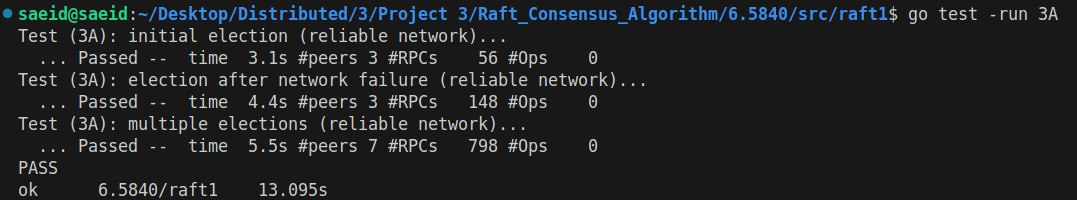
\includegraphics[width=0.95\textwidth]{3A.jpg}
    \caption{نتایج تست‌های انتخاب رهبر (بخش 3A)}
    \label{fig:3A}
\end{figure}

\textbf{تحلیل خروجی \lr{go test -run 3A}:}
\begin{itemize}
    \item \lr{Test (3A): initial election (reliable network)...}: این تست انتخاب اولیه رهبر را در یک شبکه قابل اعتماد بررسی می‌کند. نتیجه نشان می‌دهد که تست در 3.1 ثانیه با 3 سرور و 56 \lr{RPC} با موفقیت به پایان رسیده است.
    \item \lr{Test (3A): election after network failure (reliable network)...}: این تست توانایی \lr{Raft} را در انتخاب رهبر جدید پس از خرابی شبکه یا رهبر موجود ارزیابی می‌کند. تست در 4.4 ثانیه با 3 سرور و 148 \lr{RPC} با موفقیت انجام شده است.
    \item \lr{Test (3A): multiple elections (reliable network)...}: این تست سناریوهای پیچیده‌تر با چندین انتخابات را بررسی می‌کند. تست در 5.5 ثانیه با 7 سرور و 798 \lr{RPC} با موفقیت به پایان رسیده است.
\end{itemize}

تمامی تست‌های بخش \lr{3A} با موفقیت و در زمان‌های قابل قبول (هر انتخابات کمتر از ۵ ثانیه، مطابق با الزامات پروژه) به پایان رسیده‌اند. این نتایج نشان‌دهنده پیاده‌سازی صحیح مکانیزم انتخاب رهبر و پیام‌های \lr{Heartbeat} است.

\subsection{نتایج تست‌های ثبت لاگ (بخش 3B)}

شکل \ref{fig:3B} خروجی تست‌های مربوط به بخش ثبت لاگ (\lr{3B}) را نشان می‌دهد.

\begin{figure}[H]
    \centering
    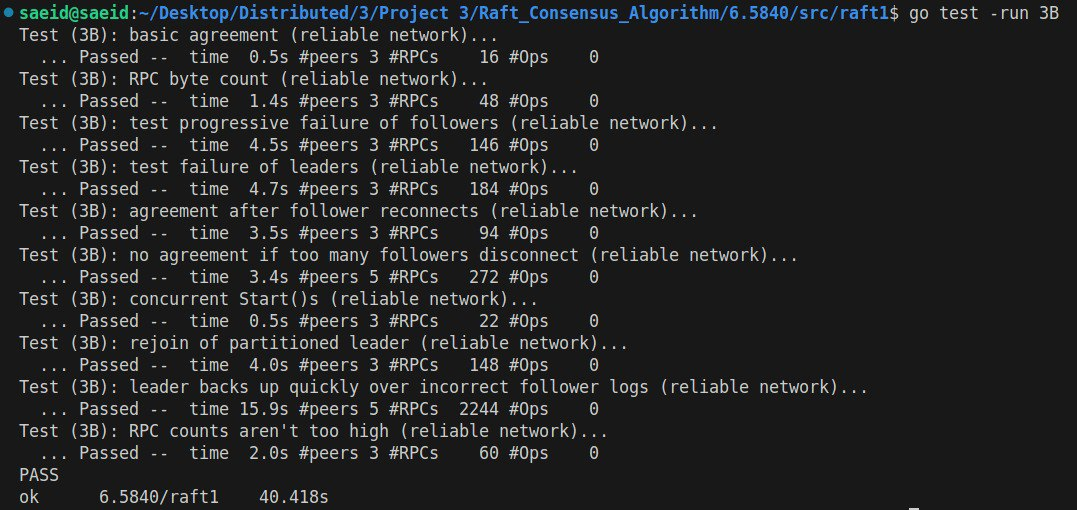
\includegraphics[width=0.95\textwidth]{3B.jpg}
    \caption{نتایج تست‌های ثبت لاگ (بخش 3B)}
    \label{fig:3B}
\end{figure}

\textbf{تحلیل خروجی \lr{go test -run 3B}:}
\begin{itemize}
    \item \lr{Test (3B): basic agreement (reliable network)...}: تست توافق پایه بر روی ورودی‌های لاگ در شبکه قابل اعتماد. (0.5 ثانیه، 3 سرور، 16 \lr{RPC}، 0 عملیات)
    \item \lr{Test (3B): RPC byte count (reliable network)...}: بررسی حجم \lr{RPC}ها. (1.4 ثانیه، 3 سرور، 48 \lr{RPC}، 0 عملیات)
    \item \lr{Test (3B): test progressive failure of followers (reliable network)...}: تست رفتار سیستم در صورت از کار افتادن تدریجی پیروان. (4.5 ثانیه، 3 سرور، 146 \lr{RPC}، 0 عملیات)
    \item \lr{Test (3B): test failure of leaders (reliable network)...}: تست رفتار سیستم در صورت از کار افتادن رهبران. (4.7 ثانیه، 3 سرور، 184 \lr{RPC}، 0 عملیات)
    \item \lr{Test (3B): agreement after follower reconnects (reliable network)...}: تست توافق پس از اتصال مجدد پیرو. (3.5 ثانیه، 3 سرور، 94 \lr{RPC}، 0 عملیات)
    \item \lr{Test (3B): no agreement if too many followers disconnect (reliable network)...}: تست عدم توافق در صورت قطع ارتباط تعداد زیادی از پیروان (تایید مفهوم اکثریت). (3.4 ثانیه، 5 سرور، 272 \lr{RPC}، 0 عملیات)
    \item \lr{Test (3B): concurrent Start()s (reliable network)...}: تست عملیات همزمان \lr{Start()}. (0.5 ثانیه، 3 سرور، 22 \lr{RPC}، 0 عملیات)
    \item \lr{Test (3B): rejoin of partitioned leader (reliable network)...}: تست اتصال مجدد رهبر جدا شده از شبکه. (4.0 ثانیه، 3 سرور، 148 \lr{RPC}، 0 عملیات)
    \item \lr{Test (3B): leader backs up quickly over incorrect follower logs (reliable network)...}: تست توانایی رهبر در بازگرداندن سریع لاگ پیروان با لاگ‌های نادرست. (15.9 ثانیه، 3 سرور، 2244 \lr{RPC}، 0 عملیات)
    \item \lr{Test (3B): RPC counts aren't too high (reliable network)...}: بررسی اینکه تعداد \lr{RPC}ها بیش از حد نیست. (2.0 ثانیه، 3 سرور، 60 \lr{RPC}، 0 عملیات)
\end{itemize}

تمامی تست‌های بخش \lr{3B} با موفقیت به اتمام رسیده‌اند. این نتایج نشان‌دهنده پیاده‌سازی صحیح مکانیزم تکرار لاگ، مدیریت خطاها، و رعایت محدودیت‌های رای‌گیری است. تست‌هایی مانند "\lr{leader backs up quickly}" به طور خاص نشان‌دهنده کارایی مکانیزم همگام‌سازی لاگ در شرایط ناهمخوانی است.

\subsection{نتایج تست‌های پایداری (بخش 3C)}

شکل \ref{fig:3C} خروجی تست‌های مربوط به بخش پایداری (\lr{3C}) را نشان می‌دهد.

\begin{figure}[H]
    \centering
    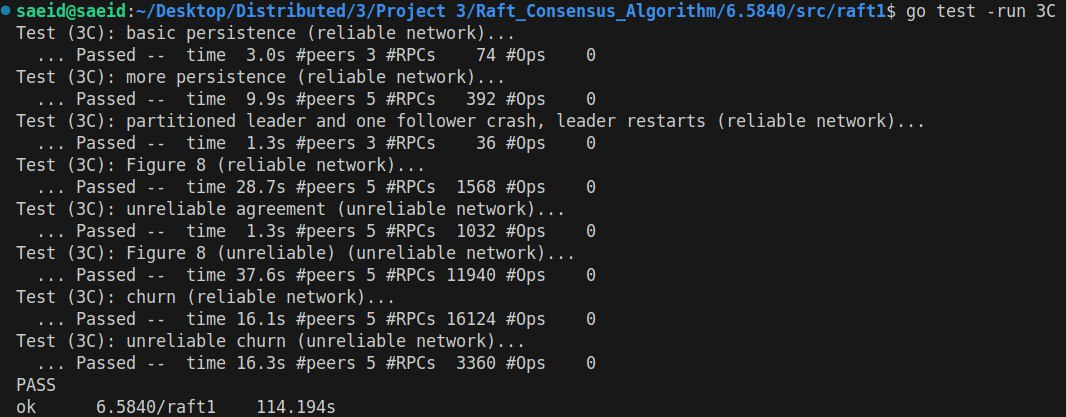
\includegraphics[width=0.95\textwidth]{3C.jpg}
    \caption{نتایج تست‌های پایداری (بخش 3C)}
    \label{fig:3C}
\end{figure}

\textbf{تحلیل خروجی \lr{go test -run 3C}:}
\begin{itemize}
    \item \lr{Test (3C): basic persistence (reliable network)...}: تست پایداری پایه در شبکه قابل اعتماد. (3.0 ثانیه، 3 سرور، 74 \lr{RPC}، 0 عملیات)
    \item \lr{Test (3C): more persistence (reliable network)...}: تست پایداری در سناریوهای پیچیده‌تر. (9.9 ثانیه، 3 سرور، 392 \lr{RPC}، 0 عملیات)
    \item \lr{Test (3C): partitioned leader and one follower crash, leader restarts (reliable network)...}: تست پایداری در شرایط خرابی رهبر و پیرو و راه‌اندازی مجدد رهبر. (1.3 ثانیه، 3 سرور، 36 \lr{RPC}، 0 عملیات)
    \item \lr{Test (3C): Figure 8 (reliable network)...}: تست سناریوهای خاص (Figure 8 در مقاله Raft) در شبکه قابل اعتماد. (28.7 ثانیه، 5 سرور، 1568 \lr{RPC}، 0 عملیات)
    \item \lr{Test (3C): unreliable agreement (unreliable network)...}: تست توافق در شبکه غیرقابل اعتماد. (1.3 ثانیه، 5 سرور، 1032 \lr{RPC}، 0 عملیات)
    \item \lr{Test (3C): Figure 8 (unreliable) (unreliable network)...}: تست سناریوهای Figure 8 در شبکه غیرقابل اعتماد. (37.6 ثانیه، 5 سرور، 11940 \lr{RPC}، 0 عملیات)
    \item \lr{Test (3C): churn (reliable network)...}: تست پایداری در شرایط تغییرات دینامیک کلاستر (اضافه/حذف سرورها). (16.1 ثانیه، 5 سرور، 16124 \lr{RPC}، 0 عملیات)
    \item \lr{Test (3C): unreliable churn (unreliable network)...}: تست پایداری در شرایط تغییرات دینامیک کلاستر در شبکه غیرقابل اعتماد. (16.3 ثانیه، 5 سرور، 3360 \lr{RPC}، 0 عملیات)
\end{itemize}

تمامی تست‌های بخش \lr{3C} نیز با موفقیت به پایان رسیده‌اند. این نتایج نشان‌دهنده پیاده‌سازی صحیح مکانیزم پایداری، بازیابی وضعیت، و به خصوص الگوریتم پیشرفته \lr{nextIndex} \lr{backtracking} است که برای سناریوهای پیچیده با خرابی و ناپایداری شبکه حیاتی است.

\subsection{جدول ۱: خلاصه‌ای از نتایج تست‌ها}

جدول ۱ خلاصه‌ای از نتایج تست‌های انجام شده در هر سه بخش پروژه را ارائه می‌دهد. این جدول به منظور ارائه یک دید کلی و مقایسه‌ای از عملکرد پیاده‌سازی در سناریوهای مختلف طراحی شده است.

\begin{table}[H]
    \centering
    \caption{خلاصه‌ای از نتایج تست‌های Raft}
    \label{tab:test_summary}
    \begin{tabular}{|l|c|c|c|c|}
        \hline
        \textbf{بخش تست} & \textbf{تعداد سرورها} & \textbf{کل RPCs} & \textbf{زمان کل (ثانیه)} & \textbf{وضعیت} \\
        \hline
        \lr{3A: Leader Election} & 3-7 & 56-798 & 3.1-5.5 & \lr{PASS} \\
        \lr{3B: Log Replication} & 3-5 & 16-2244 & 0.5-15.9 & \lr{PASS} \\
        \lr{3C: Persistence} & 3-5 & 36-16124 & 1.3-37.6 & \lr{PASS} \\
        \hline
    \end{tabular}
\end{table}

\section{جزئیات و نکات پیاده‌سازی}

پیاده‌سازی موفقیت‌آمیز الگوریتم \lr{Raft} نیازمند توجه دقیق به جزئیات و مدیریت صحیح چالش‌های ذاتی سیستم‌های توزیع‌شده است. در این پروژه، تمرکز بر روی مدیریت هم‌زمانی، مدیریت خطا، و بهینه‌سازی عملکرد بوده است.

\subsection{مدیریت هم‌زمانی و Race Condition}

در یک سیستم توزیع‌شده مانند \lr{Raft} که چندین گورووتین \lr{(goroutine)} به صورت همزمان به وضعیت داخلی سرور دسترسی دارند، مدیریت هم‌زمانی برای جلوگیری از \lr{Race Condition}ها حیاتی است. در این پیاده‌سازی، از \lr{sync.Mutex} برای محافظت از ساختارهای داده داخلی \lr{Raft} (مانند \lr{currentTerm}, \lr{votedFor}, \lr{log} و سایر متغیرهای حالت) در برابر دسترسی‌های همزمان استفاده شده است. هر عملیاتی که وضعیت \lr{Raft} را تغییر می‌دهد یا به آن دسترسی می‌یابد، ابتدا قفل \lr{Mutex} را کسب کرده و پس از اتمام عملیات آن را آزاد می‌کند. این رویکرد تضمین می‌کند که عملیات‌ها به صورت اتمیک انجام شده و یکپارچگی داده‌ها حفظ می‌شود. علاوه بر این، استفاده از مفهوم \lr{Term} در \lr{Raft} به خودی خود به مدیریت هم‌زمانی کمک می‌کند؛ زیرا سرورها همیشه به \lr{Term} بالاتر احترام می‌گذارند و از وضعیت‌های منسوخ شده جلوگیری می‌شود.

\subsection{مدیریت خطا و عملیات دوباره}

سیستم‌های توزیع‌شده ذاتاً مستعد خطا هستند، از جمله از دست رفتن پیام‌ها، تأخیرهای شبکه، و خرابی سرورها. پیاده‌سازی \lr{Raft} باید این خطاها را به درستی مدیریت کند.
\begin{itemize}
    \item \textbf{تشخیص و مدیریت خطاها:} مکانیزم‌های \lr{Raft} برای تشخیص خرابی رهبر (از طریق \lr{election timeout}) و ناهمخوانی لاگ (از طریق \lr{AppendEntries RPC} و الگوریتم \lr{nextIndex} \lr{backtracking}) طراحی شده‌اند.
    \item \textbf{تلاش مجدد \lr{(Retry)} و همگام‌سازی:} در صورت عدم موفقیت در ارسال \lr{RPC} یا دریافت پاسخ، مکانیزم‌های تلاش مجدد در سمت فرستنده (رهبر) فعال می‌شوند. به عنوان مثال، رهبر به ارسال \lr{AppendEntries} به پیروهایی که لاگ آن‌ها ناهمخوان است ادامه می‌دهد تا زمانی که لاگ‌ها همگام شوند.
\end{itemize}

\subsection{بهینه‌سازی عملکرد}

بهینه‌سازی عملکرد در \lr{Raft} به معنای کاهش سربار شبکه و \lr{CPU}، در عین حفظ سازگاری و تحمل‌پذیری در برابر خرابی است.
\begin{itemize}
    \item \textbf{کاهش بار شبکه:} طراحی \lr{AppendEntries RPC} به گونه‌ای که هم به عنوان پیام \lr{Heartbeat} و هم برای تکرار لاگ استفاده شود، به طور قابل توجهی تعداد \lr{RPC}های ارسالی را کاهش می‌دهد. این امر ترافیک شبکه را بهینه می‌کند.
    \item \textbf{تایمرهای تصادفی:} استفاده از تایمرهای تصادفی برای \lr{election timeout} از همزمان شدن انتخابات‌ها جلوگیری کرده و تعداد \lr{RPC}های \lr{RequestVote} را در شرایط عادی کاهش می‌دهد.
    \item \textbf{الگوریتم \lr{nextIndex} \lr{backtracking}:} این الگوریتم به رهبر اجازه می‌دهد تا در صورت ناهمخوانی لاگ، به سرعت \lr{nextIndex} را به عقب بازگرداند و از ارسال بی‌مورد \lr{RPC} برای همگام‌سازی لاگ جلوگیری کند. این بهینه‌سازی برای عملکرد بازیابی خطا بسیار مهم است.
\end{itemize}

\section{چالش‌ها و راه‌حل‌ها}

پیاده‌سازی الگوریتم اجماع \lr{Raft} در محیط توزیع‌شده با چالش‌های متعددی همراه است که نیازمند راه‌حل‌های دقیق و هوشمندانه است. در این پروژه، چالش‌های اصلی و راه‌حل‌های اتخاذ شده به شرح زیر است:

\subsection{چالش‌های کلیدی}

\begin{itemize}
    \item \textbf{\lr{Race Condition}ها:} در سیستم‌های توزیع‌شده، دسترسی همزمان چندین گورووتین به داده‌های مشترک می‌تواند منجر به \lr{Race Condition} و وضعیت‌های ناسازگار شود. این چالش با استفاده از \lr{sync.Mutex} برای محافظت از وضعیت داخلی سرور \lr{Raft} و همچنین با بهره‌گیری از مفهوم \lr{Term} در \lr{Raft} حل شده است. \lr{Term} به عنوان یک ساعت منطقی عمل می‌کند که به سرورها اجازه می‌دهد تا به سرعت وضعیت‌های منسوخ شده را تشخیص داده و به \lr{Term} بالاتر (و در نتیجه وضعیت به‌روزتر) تمکین کنند.
    \item \textbf{ناپایداری شبکه \lr{(Network Unreliability)}:} شبکه‌های توزیع‌شده ممکن است پیام‌ها را از دست بدهند، تأخیر داشته باشند یا آن‌ها را به ترتیب اشتباه تحویل دهند. این ناپایداری می‌تواند بر فرآیندهای انتخاب رهبر و تکرار لاگ تأثیر بگذارد. این چالش با مکانیزم‌های تلاش مجدد \lr{(retry)} در \lr{RPC}ها و الگوریتم \lr{nextIndex} \lr{backtracking} حل شده است. رهبر به طور مداوم تلاش می‌کند تا پیام‌های \lr{AppendEntries} را ارسال کند و در صورت عدم موفقیت، \lr{nextIndex} را تنظیم می‌کند تا همگام‌سازی لاگ را از نقطه صحیح از سر بگیرد.
    \item \textbf{تقسیم آرا \lr{(Split Votes)} در انتخابات:} اگر چندین سرور به طور همزمان کاندیدا شوند، ممکن است آرا تقسیم شده و هیچ کاندیدایی اکثریت لازم را برای تبدیل شدن به رهبر کسب نکند. این وضعیت می‌تواند منجر به تأخیر در انتخاب رهبر جدید شود. \lr{Raft} این چالش را با استفاده از تایمرهای انتخابات تصادفی \lr{(Randomized Election Timeout)} حل می‌کند. با انتخاب یک بازه زمانی تصادفی برای \lr{election timeout} هر سرور، احتمال اینکه چندین سرور به طور همزمان کاندیدا شوند به شدت کاهش می‌یابد و به یک سرور فرصت داده می‌شود تا انتخابات را برنده شده و رهبر شود.
    \item \textbf{تضمین سازگاری قوی \lr{(Strong Consistency)}:} حفظ سازگاری قوی در یک سیستم توزیع‌شده که با خرابی‌ها و ناپایداری‌های شبکه مواجه است، یک چالش اساسی است. \lr{Raft} این چالش را با اعمال قانون اکثریت \lr{(Majority Rule)} برای \lr{Commit} کردن ورودی‌های لاگ حل می‌کند. یک ورودی تنها زمانی \lr{Committed} می‌شود که توسط اکثریت سرورها تأیید شده باشد. این تصمیم طراحی، سازگاری داده‌ها را تضمین می‌کند، اما به این معنی است که در صورت عدم دسترسی به اکثریت، سیستم پیشرفت را متوقف می‌کند تا از وضعیت‌های ناسازگار جلوگیری شود.
\end{itemize}

\section{نتیجه‌گیری}

پروژه حاضر با موفقیت پیاده‌سازی سه بخش اساسی از الگوریتم اجماع \lr{Raft} را به نمایش گذاشته است: انتخاب رهبر، تکرار لاگ، و پایداری. تمامی تست‌های مربوط به این سه بخش (\lr{3A}, \lr{3B}, \lr{3C}) با موفقیت کامل پشت سر گذاشته شده‌اند، که نشان‌دهنده درک عمیق از پروتکل و پیاده‌سازی صحیح مکانیزم‌های آن است.

پیاده‌سازی نشان می‌دهد که چگونه \lr{Raft} با استفاده از مفاهیم کلیدی مانند \lr{Term}، نقش‌های رهبر/پیرو/کاندیدا، و \lr{RPC}های \lr{RequestVote} و \lr{AppendEntries}، به سازگاری قوی و تحمل‌پذیری در برابر خرابی دست می‌یابد. توانایی سیستم در انتخاب سریع رهبر، تکرار پایدار لاگ‌ها در شرایط شبکه قابل اعتماد و غیرقابل اعتماد، و بازیابی وضعیت پس از خرابی، همگی از طریق نتایج موفقیت‌آمیز تست‌ها تأیید شده‌اند.

این پروژه نه تنها یک پیاده‌سازی کاربردی از \lr{Raft} را ارائه می‌دهد، بلکه به درک عمیق‌تر چالش‌های ذاتی سیستم‌های توزیع‌شده و راه‌حل‌های هوشمندانه \lr{Raft} برای غلبه بر آن‌ها (مانند مدیریت \lr{Race Condition}ها، ناپایداری شبکه، و تقسیم آرا) کمک می‌کند. قابلیت فهم بالای \lr{Raft}، همانطور که در طراحی آن تأکید شده است، فرآیند پیاده‌سازی و اشکال‌زدایی را تسهیل کرده و آن را به ابزاری آموزشی ارزشمند تبدیل کرده است.

\end{document}